\pdfminorversion=4
\documentclass[final]{beamer}
\usetheme{Madrid}

\usepackage[orientation=portrait,size=a2,scale=1.4,debug]{beamerposter}
\usepackage[absolute,overlay]{textpos}
\setlength{\TPHorizModule}{1cm}
\setlength{\TPVertModule}{1cm}
\usepackage{tikz}
\usepackage[style=numeric,firstinits=true,sorting=none,doi=false,isbn=false,url=false,eprint=false,backend=bibtex]{biblatex}
\bibliography{references.bib}
\setbeamertemplate{bibliography item}[text]
%\renewcommand*{\bibfont}{\tiny}
\renewbibmacro{in:}{}
\AtEveryBibitem{\clearfield{title}}
\AtEveryBibitem{\clearfield{pages}}
\setbeamertemplate{bibliography item}[text]
\usepackage[labelfont={color={darkblue}},font=scriptsize,labelformat=simple]{caption}
\usepackage{setspace}

\setbeamertemplate{navigation symbols}{}  % no navigation on a poster
\setbeamertemplate{caption}[numbered]

\setbeamertemplate{itemize subitem}{\tiny\raise1.5pt\hbox{\donotcoloroutermaths$\blacktriangleright$}}
\setbeamertemplate{itemize subsubitem}{\tiny\raise1.5pt\hbox{\donotcoloroutermaths$\blacktriangleright$}}
\setbeamerfont*{itemize/enumerate body}{size=\footnotesize}
\setbeamerfont*{itemize/enumerate subbody}{parent=itemize/enumerate body,size=\scriptsize}
\setbeamerfont*{itemize/enumerate subsubbody}{parent=itemize/enumerate body,size=\scriptsize}

\definecolor{lightblue}{rgb}{0.0,0.45,0.81}
\definecolor{lighterblue}{rgb}{0.415,0.678,0.894}
\definecolor{darkblue}{rgb}{0,0.243,0.447}
\definecolor{vdarkblue}{rgb}{0,0.162,0.298}
\setbeamercolor{frametitle}{bg=lightblue,fg=white}
\setbeamerfont{normal text}{family=helvet}
\setbeamerfont{local structure}{family=helvet}

\setbeamercolor*{author in head/foot}{bg=darkblue}
\setbeamercolor*{logo in head/foot}{bg=darkblue,fg=white}
\setbeamercolor*{title in head/foot}{bg=lightblue,fg=vdarkblue}
\setbeamercolor*{date in head/foot}{bg=darkblue,fg=white}
\setbeamercolor{title}{bg=darkblue}
\setbeamercolor{headline}{bg=lightblue,fg=white}
\setbeamercolor{frametitle}{bg=darkblue}
\setbeamercolor{under headline}{bg=lighterblue,fg=darkblue}
\setbeamercolor{footline}{bg=darkblue}
\setbeamercolor{block title}{bg=lighterblue,fg=vdarkblue}
\setbeamercolor{lower separation line head}{bg=darkblue}

\setbeamerfont*{title in head/foot}{size*={44}{44}}
\setbeamerfont*{date in head/foot}{size*={28}{28}}
\setbeamerfont*{bibliography item}{size*={24}{24}}
\setbeamerfont*{bibliography entry journal}{size*={36}{36}}
\setbeamerfont*{footline}{size*={44}{44}}

\setbeamersize{text margin left=44mm}
\setbeamersize{text margin right=44mm} 

\setbeamertemplate{headline}
{
  \leavevmode%
  \vskip0.015\paperwidth
  \hskip0.015\paperwidth \hbox{%
  \begin{beamercolorbox}[wd=.285\paperwidth,ht=2.5cm,center,dp=1ex]{logo in
    head/foot}%
  \usebeamerfont{logo in head/foot}\includegraphics[width=.25\paperwidth]{./UClogo_bg_transparent.png}%
\end{beamercolorbox}%
  \begin{beamercolorbox}[wd=.685\paperwidth,dp=1ex,right,ht=2.5cm]{date in head/foot}%
    \usebeamerfont{date in head/foot}MPhil in Scientific
    Computing\hspace{1cm}\vspace{0.05cm}
\hskip0.015\paperwidth
\end{beamercolorbox}%
}%
  \vskip0pt%
\hbox{%
\hskip0.015\paperwidth
  \begin{beamercolorbox}[wd=0.97\paperwidth,dp=1ex,ht=2.5cm,center]{under headline}%
    \usebeamerfont{title in head/foot}%
    \begin{centering}\inserttitle\end{centering}\vspace{0.05cm}%
  \end{beamercolorbox}%
\hskip0.015\paperwidth
}%
%  \vskip0pt%
\hbox{%
\hskip0.015\paperwidth
  \begin{beamercolorbox}[wd=0.97\paperwidth,dp=0.5ex,center]{lower separation line head}%
    \rule{0pt}{2pt}%
  \end{beamercolorbox}%
\hskip0.015\paperwidth
}%
%  \vskip0pt%
}


\setbeamertemplate{block begin}{
  \usebeamerfont*{block title}

  \begin{beamercolorbox}[ht = 2.0cm, sep=0.25cm,leftskip=0.5cm]%,, colsep*=.75ex]
  {block title}%
  \usebeamerfont*{block title}\insertblocktitle \vphantom{Pp}
  \end{beamercolorbox}%
  {\ifbeamercolorempty[bg]{block body}{}{\nointerlineskip\vskip-0.5pt}}%
  \usebeamerfont{block body}%
  \begin{beamercolorbox}[sep=0.75cm]%[colsep*=.75ex,vmode]
  {block body}%
    %\ifbeamercolorempty[bg]{block body}{\vskip-.25ex}{\vskip-.75ex}\vbox{}%
  }
  \setbeamertemplate{block end}{
  \end{beamercolorbox}
  \vspace{0.6cm}
}


\setbeamertemplate{frametitle}
{
  \leavevmode%
  \begin{beamercolorbox}[wd=\paperwidth,ht=1cm]{frametitle}
   \hspace{1em}\insertframetitle\vspace{0.35cm}
   \end{beamercolorbox}%
   %\vskip-0.4cm%
  \begin{beamercolorbox}[wd=\paperwidth,ht=1ex]{under headline}%
    \end{beamercolorbox}%
}

%%% USER MODIFIABLE PARTS START BELOW %%%

\setbeamertemplate{footline}{  
  \leavevmode%
  \hbox{%
\hskip0.015\paperwidth
  \begin{beamercolorbox}[wd=.235\paperwidth,dp=1ex,right,ht=2.5cm]{date in head/foot}%
    \usebeamerfont{date in head/foot}\centering\insertauthor\vspace{0.65cm}
\end{beamercolorbox}%
  \begin{beamercolorbox}[wd=.45\paperwidth,ht=2.5cm,center,dp=1ex]{logo in head/foot}%
%% EDIT YOUR SPONSOR LOGO BELOW %%
  \usebeamerfont{logo in head/foot}
%\includegraphics[height=2cm]{./sponsor.png}%
 \vspace{0.1cm}
\end{beamercolorbox}%

\begin{beamercolorbox}[wd=0.285\paperwidth,ht=2.5cm,dp=1ex,center]{date
    in head/foot}%
%% EDIT YOUR SUPERVISOR'S NAME BELOW %%
\hspace{-4cm}
  \usebeamerfont{date in head/foot}{Supervisor: Dr. Maria Nikodemou}\vspace{0.6cm}
  \end{beamercolorbox}}%
\hskip0.015\paperwidth
  \vskip0.015\paperwidth%
  }

% EDIT FONT SIZE FOR BLOCKS HERE

\setbeamerfont*{caption name}{size=\fontsize{24pt}{28pt}}
\setbeamerfont*{caption}{size=\fontsize{24pt}{28pt}}
\setbeamerfont*{block body}{size=\fontsize{24pt}{28pt}}
\setbeamerfont*{block title}{size=\fontsize{36pt}{40pt}}

%% EDIT TITLE AND AUTHOR

\title{Magnetohydrodynamic Simulation in Complex Geometries }
\author{Silong Li}

\begin{document}
\begin{frame}{} 

\begin{textblock}{19.5}(1,7.5)
\begin{block}{Overview}
The study explores the interaction between plasma and the resistive wall, with a focus on implementing the outcomes model through simulations under tokamaks scenario. After a brief introduction, the boundary conditions for perfect conducting walls, insulating walls, and resistive walls are mathematically derived and numerically approximated. These boundary conditions are then applied in validation tests. Ultimately, a comprehensive model is utilized for plasma simulations within a resistive tokamak vessel.
\end{block}
\begin{block}{Methodology}
A ideal MHD model is applied on modeling the core plasma. 
%\begin{align*}
%	\frac{\partial \rho}{\partial t} + \nabla \cdot (\rho \mathbf{v}) &= 0 \\
%	\frac{\partial (\rho \mathbf{v})}{\partial t} + \nabla \cdot \left[ \rho \mathbf{v} \otimes \mathbf{v} + \left( p + \frac{1}{2}\mathbf{B}^2 \right) \mathbf{I} - \mathbf{B} \otimes \mathbf{B} \right] &= 0 \\
%	\frac{\partial U}{\partial t} + \nabla \cdot \left[ \left( U + p + \frac{1}{2}\mathbf{B}^2 \right) \mathbf{v} - (\mathbf{v} \cdot \mathbf{B}) \mathbf{B} \right] &= 0 \\
%	\frac{\partial \mathbf{B}}{\partial t} + \nabla \cdot (\mathbf{B} \otimes \mathbf{v} - \mathbf{v} \otimes \mathbf{B}) &= 0
%\end{align*}
A first-order MHD-HLLC solver is utilized and extended to second-order accuracy through the application of the MUSCL-Hancock scheme. Mixed divergence cleaning is applied to correct the non-zero divergence arising from plasma-wall interactions, details in \cite{vides2013divergence}. 

\end{block}
\begin{block}{Boundary Conditions}
In the selection of boundary conditions, different approaches are applied to the hydrodynamic effects and the magnetic field. On hydrodynamics effect, reflective Dirichlet condition is applied on velocity field and Neumann condition on scalar variables. For details, in \cite{sambasivan2009ghost}.
On magnetic field, there mainly three boundary conditions:
\vspace{0.5cm}

\textbf{Perfect conducting wall}
\begin{align*}
	\begin{aligned}
		\frac{\partial \left(\mathbf{n}\cdot\mathbf{B}\right)}{\partial t}= 0
	\end{aligned}
	\ \ \ 
	& \Rightarrow 
	\ \ \ 
	\begin{aligned}
		B_n=B_{n0}&\ \ \text{Dirichlet}\ \\
		{\partial B_t}/{\partial \mathbf{n}}=0&\ \ \text{Neumann}
	\end{aligned}
\end{align*}

\vspace{0.3cm}
\textbf{Insulating wall}
\begin{align*}
	\begin{aligned}
		\nabla \times \mathbf{B} &= 0 \\
		\nabla \cdot \mathbf{B} &= 0
	\end{aligned}
	\ \ \ 
	& \Rightarrow 
	\ \ \ 
	\begin{aligned}
		\partial B_n/\partial \mathbf{n} = 0&\ \ \text{Neumann}\\
		{\partial B_t}/{\partial \mathbf{n}}=0&\ \ \text{Neumann}
	\end{aligned}
\end{align*}

\vspace{0.5cm}
\textbf{Resistive wall}
\begin{align*}
\frac{\partial \mathbf{B}}{\partial t}+\eta_{w}\nabla\times\nabla\times\mathbf{B}=0
\label{equ:magneticDiffusion},
\end{align*}
updated using ghost fluid method.
\end{block}


\end{textblock}

% Second column

\begin{textblock}{19.5}(21.5,7.5)
\begin{block}{Plasma in Resistive Tokamak Vessel}
The following graph shows $B_z$ in simulation within a resistive tokamak-shaped vessel. This figure is taken from the moment $t=0.2$ after the core dense plasma hitting the vessel wall with resistivity $\eta_w=0.05$. The interaction on magnetic field between plasma and vessel wall result in significant increase in $B_z$ on wall.\\
\begin{figure}
\begin{minipage}{0.90\linewidth}
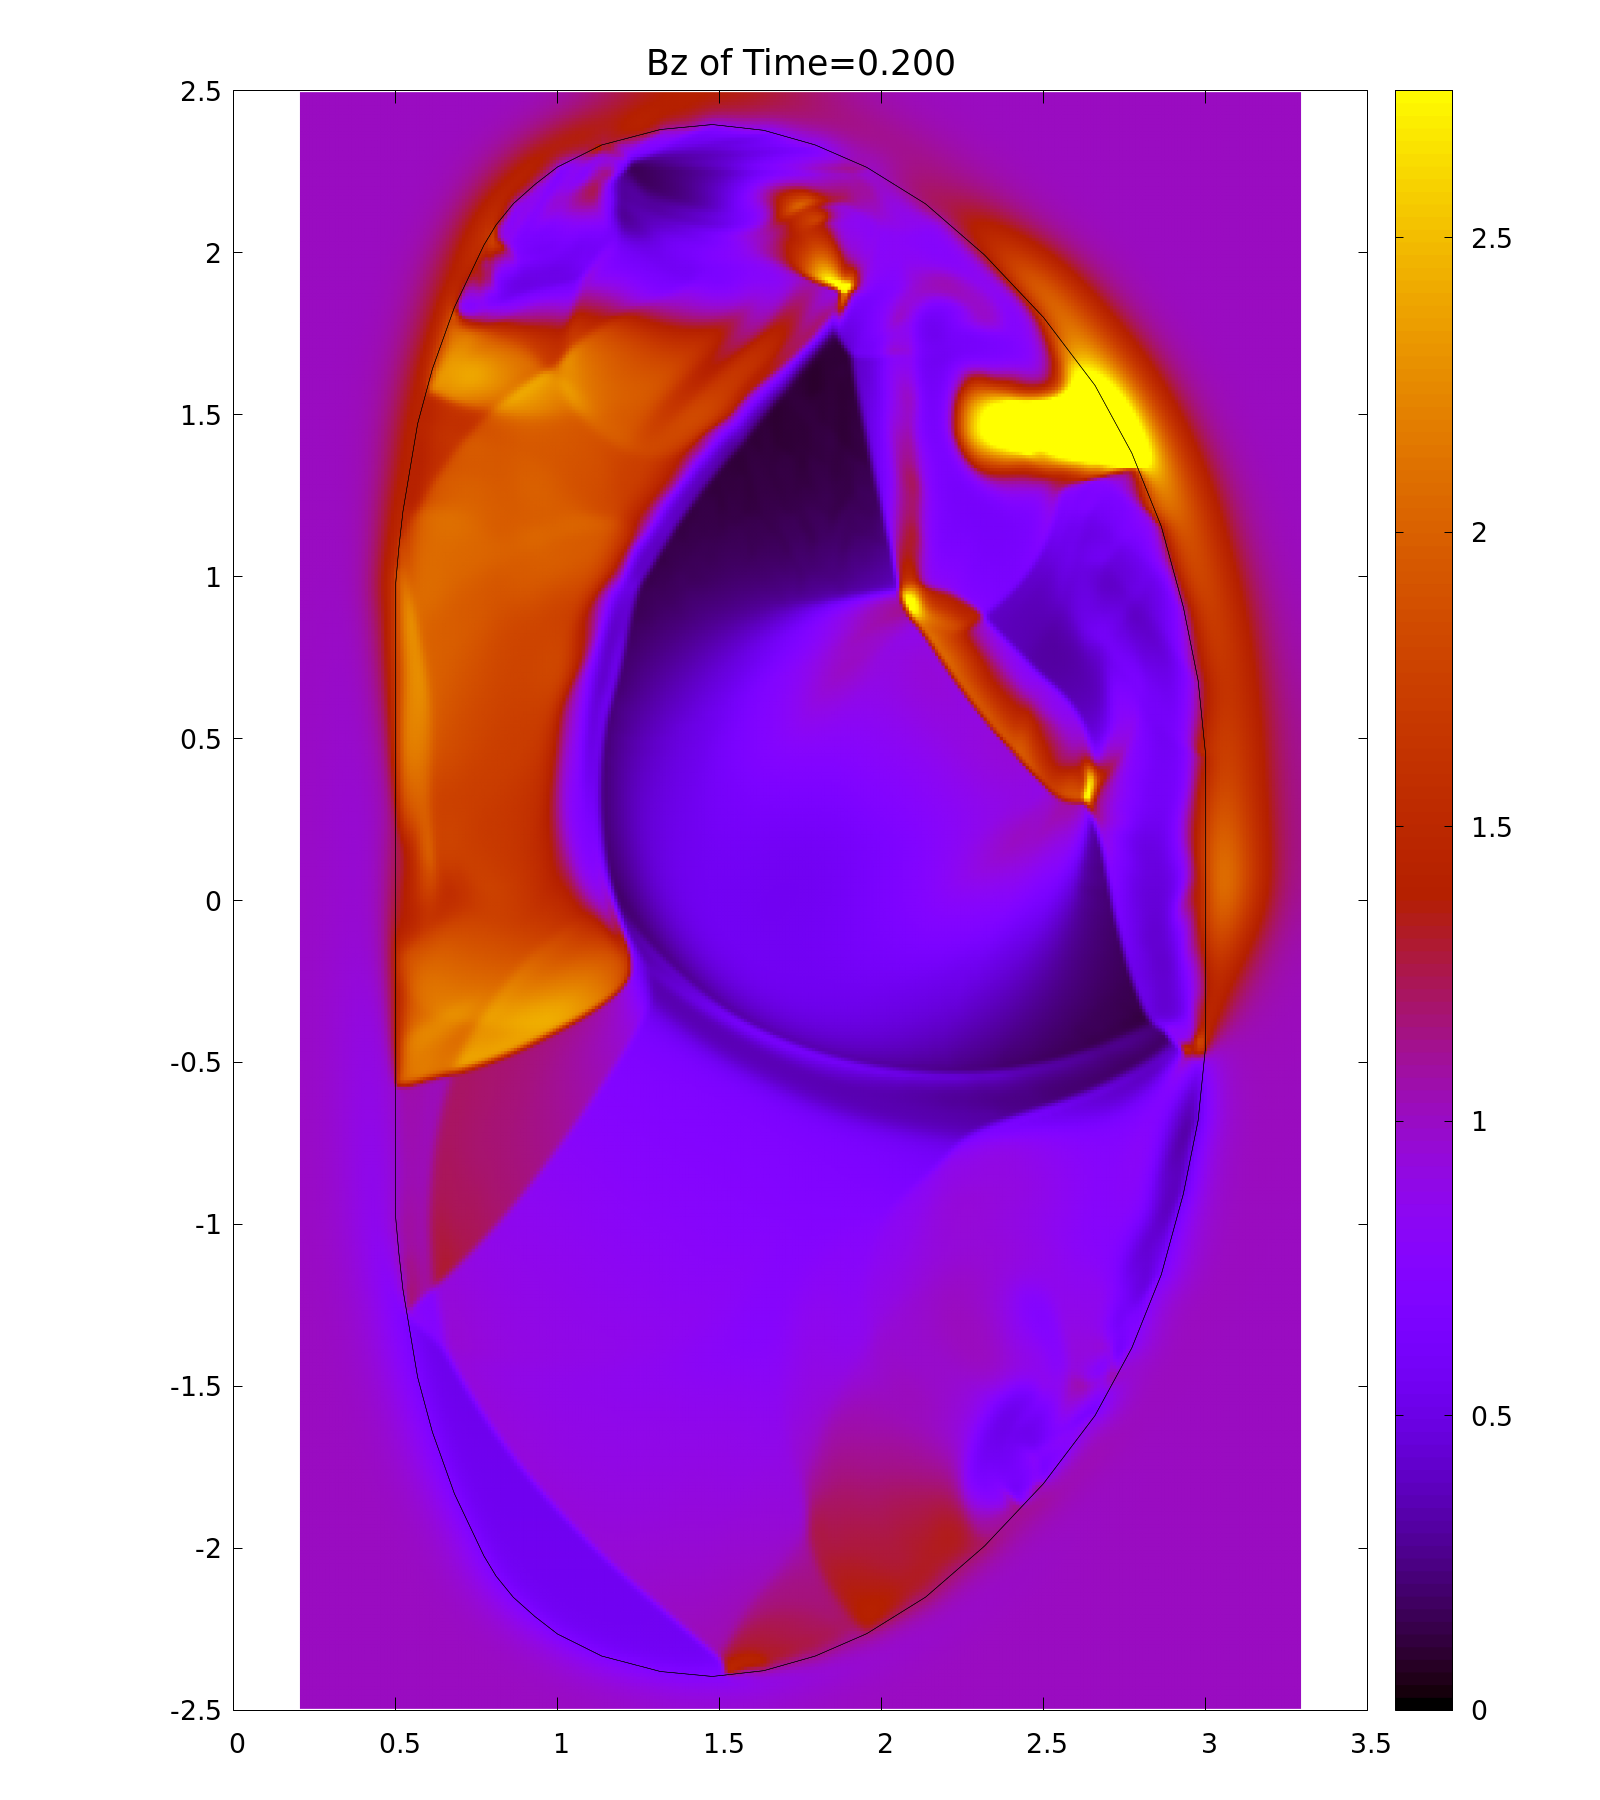
\includegraphics[width = \linewidth]{Poster_Bz_100.png}
\end{minipage}\\
\begin{minipage}{0.95\linewidth}
\caption{$B_z$ of plasma in a cylindrical equilibrium test within a tokamak-shaped vessel, outlined by a thin black line. It is taken after the core plasma hitting $\eta_{w}=0.05$ resistive wall. Interaction between plasma and wall result in some penetration on wall.}
\label{fig:CoffeeFig}
\end{minipage}
\end{figure}
\end{block}

\vspace{-0.2cm}
\begin{block}{Consistent Equation}
	After discussion on boundary condition consistency, a consistent equation across conditions is proposed
	\begin{equation*}
		\nabla^2\mathbf{B}=\frac{nq_e^2}{m\nu}\frac{\partial \mathbf{B}}{\partial t}-\frac{nq_e^2}{m\nu}e^{-\nu t}\frac{\partial \mathbf{B}}{\partial t}
	\end{equation*}
\end{block}

\vspace{-0.2cm}
\begin{block}{References and Acknowledgements}
\begin{minipage}{0.9\linewidth}
     {     \printbibliography   % i.e. the references.bib file
     } 
\end{minipage}
\vspace{2ex}

Thanks to my supervisor, Dr. Maria Nikodemou.
\end{block}

\end{textblock}

\end{frame}
\end{document}
